\documentclass[12pt,letterpaper,titlepage, final]{report}

\usepackage{fontspec}
\defaultfontfeatures{Mapping=tex-text}
\usepackage{xunicode}
\usepackage{xltxtra}
\usepackage{amsmath}
\usepackage{pdfpages}
\usepackage{amsfonts}
\usepackage{bbold}
\usepackage{amssymb}
\setcounter{secnumdepth}{0}
\usepackage{nameref}
\usepackage{enumitem}
\usepackage{environ}
\usepackage{pgfplots}
\usepackage{listings}

\usepackage{hyperref}
\hypersetup{
    colorlinks=true,
    linkcolor=blue,
    filecolor=magenta,      
    urlcolor=cyan,
}
\urlstyle{same}

\showboxdepth=\maxdimen
\showboxbreadth=\maxdimen


\usepackage{paracol}
\usepackage{wrapfig}
\globalcounter{table}
\globalcounter{figure}
\usepackage{graphicx}
\usepackage[left=1in,right=1in,top=1in,bottom=1in]{geometry}
\graphicspath{{img/}}

\author{Jacob Abel}
\title{	Final Project Specification
	\\\large ECE4514 CRN:13112
}

\setlength{\parskip}{0.5em}

\begin{document}
\maketitle
\begin{raggedright}
\hypertarget{projobj}{\section{Project Objectives}}

This project intends to provide a deliverable of a Synthesisable SystemVerilog GameBoy DMG emulator. With consideration for the time constraints, this emulator will be able to run the game "Pokemon Red" with some limitations. The serial link cable and infra-red communication subsystems will not be implemented so there will be no support for any multi-device interactions. Additionally, the device resets will be divided into soft and hard resets. Soft resets will not reset the save Catridge/MBC RAM while hard resets will. The controller will be emulated by a PS/2 keyboard and the 160x144 LCD display will be up-scaled to 800x720 and rendered on a 1024x768 VGA display running at 60Hz. The hardware and controls will map as shown below.
\vfill
\begin{figure}[ht]
\centering
\begin{tabular}{|r|c|c|c|c|c|c|c|c|}
\hline 
\textbf{Controller:} & Up & Left & Down & Right & A & B & Start & Select \\ 
\hline 
\textbf{Keyboard:} & W & A & S & D & Space & Escape & Tab & Tilde \\ 
\hline 
\end{tabular} 
\hypertarget{fig1}{\caption{Controller$\mapsto$Keyboard Mappings}}
\end{figure}
\vspace{2\baselineskip}
\begin{figure}[ht]
\centering
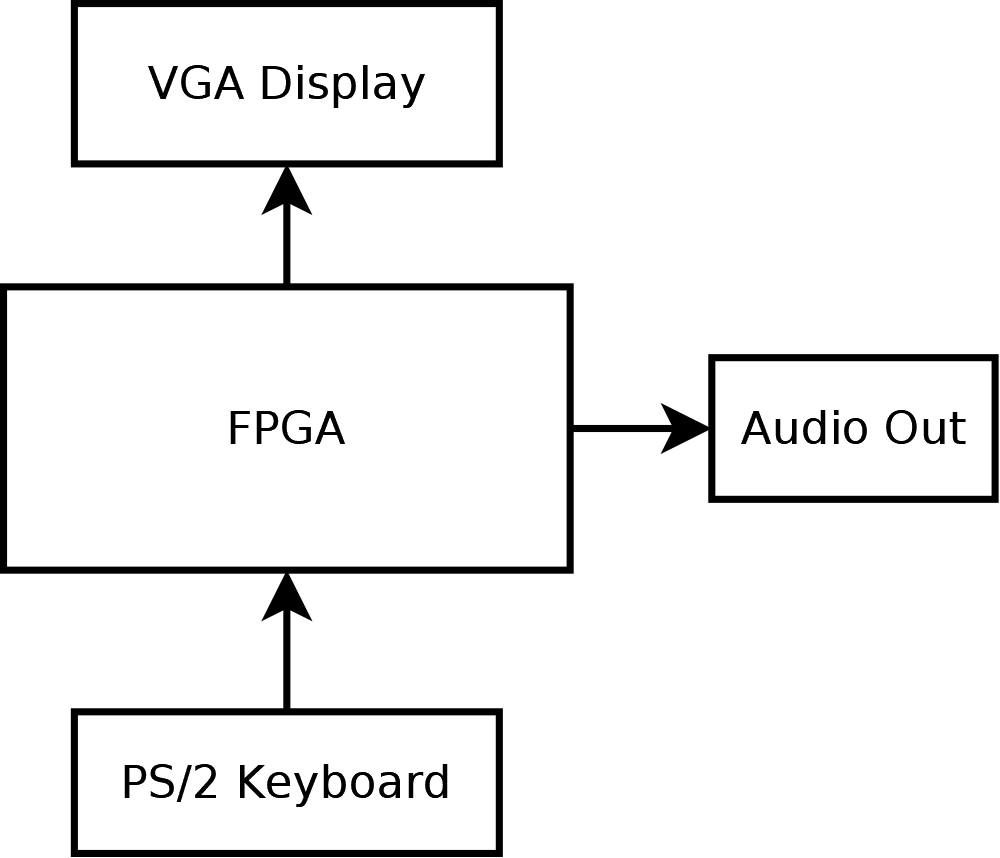
\includegraphics[width=\textwidth, height=20\baselineskip, keepaspectratio=true]{GB_Dia}
\hypertarget{fig2}{\caption{Physical Hardware Layout}}
\end{figure}


\clearpage

\hypertarget{desdesc}{\section{Design Description}}

The final design will replicate the operation of the GameBoy DMG handheld console for use with the game "Pokemon Red" with reasonable accuracy and within the scope outlined in \hyperlink{projobj}{Project Objectives}. The design description below offers an initial starting point however the design is free to be restructured as necessary provided that all required observable behaviour is replicated and a final updated project specification is offered detailing the up-to-date structuring of the deliverable.

\subsection{PS/2 Module}

The PS/2 submodule is an adaptor for the PS/2 Keyboard and will map keyboard keys to the game boy controller button outputs as detailed in \hyperlink{fig1}{Figure 1}. The adaptor will use a PS/2 IP core for handling the protocol.

\subsection{DAC Module}

The DAC submodule mostly reuses the audio modules from prior assignments with modifications as necessary to integrate with and upscale the LCD display output.

\subsection{VGA Module}

The VGA submodule reuses the XGA modules from prior assignments with modifications as necessary to facilitate the vertical and horizontal interrupts on the primary DMG module.

\subsection{RAM \& VRAM Modules}

These modules instantiate the Work RAM and Video RAM for the DMG module. These modules instantiate 64 kilobits/8 kilobytes of Work RAM and VRAM. The VRAM(in conjunction with the OAM RAM discussed later) stores all of the visual sprites and textures as well as coordinate maps necessary for the LCD Controller to generate the final rendered display. The Work RAM on the other hand is a general RAM for the instructions executing on the CPU core.

\subsection{Memory Bank Controller Module}

This module implements the MBC3 controller with 1 megabyte of ROM (for the game code) and 32 kilobytes of RAM as well. The RAM and ROM can be addressed by the CPU and the data stored in RAM persists through soft reset. This is because this particular MBC3 module that is being emulated has an onboard battery to maintain the RAM contents. As such, this is where save data is persisted.

\subsection{Gameboy DMG Module}

This is the primary submodule of the project. It will replicate the functionality of the DMG as specified by the accompanying GameBoy DMG documentation in \hyperlink{annexa}{Annex A} and \hyperlink{annexc}{Annex C}. This module will contain the submodules for each module present in \hyperlink{fig4}{Figure 4}. Because of the broad yet relatively shallow nature of this module, only the major functionality of each primary subsystem will be outlined beyond what is already provided in \hyperlink{annexa}{Annex A}.

\subsubsection{CPU Core}

The CPU core is largely similar to the Intel 8080 and Zilog Z80 CPUs however it has some major differences as outlined in \hyperlink{cpucomp}{CPU Comparision with Z80}. For the most part it is a Zilog Z80 running at 4MHz with all instruction execution times being rounded up to 4 clock cycles. An additional element of note is that there is a small internal RAM for periods where the primary data bus is in use. The rest of the CPU operations are detailed under \hyperlink{annexa}{Annex A} and \hyperlink{page.28}{Chapter 1.2} and \hyperlink{page.103}{Chapter 4} of Annex C.

\subsubsection{Memory Subsystem}

The memory map subsystem is effectively an IOMMU or IO memory management unit. This system controls which device is accessed or written to when a specific memory address is accessed. \hyperlink{memmap}{The Memory Map section of Annex A} details which subsystem is routed to by each address range. Primarily, the important addressable ranges are the MBC ROM, MBC RAM, Work RAM, and IO Registers. The full details for each of the registers is available in \hyperlink{annexa}{Annex A} and \hyperlink{annexc}{Annex C}. This module will primarily be composed of a large range select chain and routing outputs.

\subsubsection{Sound Subsystem}

The Audio subsystem is divided into six parts: the four audio generators, a small RAM, and a signal mixer. Audio generators one and two produce pulse width tone patterns, generator three is a static noise generator. It creates either clean or dirty static. Audio generator four produces a looping waveform based on the contents of the small RAM. The RAM obviously holds audio data. Finally, the signal mixer combines all four signals and outputs it to the DAC subsystem. More details are available in \hyperlink{soundhardware}{Audio Subsystem Hardware}, \hyperlink{soundcontrol}{Audio Subsystem Control}, and \hyperlink{page.87}{Chapter 3 of Annex C}.

\clearpage

\subsubsection{Timer Subsystem}
This subsystem is divided into the divider and timer functionalities. The divider is a clock divider circuit that controls the rate at which the timer is incremented. The divider counter increments at 16384Hz and can be used to drive the timer at 4096Hz, 16384Hz, 65536Hz, and 262144 Hz. The timer is 8 bit timer that when it overflows is reset with a specified value and can trigger an interrupt. Further details on timer operation can be found under \hyperlink{timer}{Timer Behaviour in Annex A} or \hyperlink{page.35}{Sections 2.4.2 and 2.4.3 of Annex C}

\subsubsection{Interrupt Subsystem}
The interrupt subsystem controls all hardware interrupts in the system. On a signal from one of the connected subsystems it suspends execution of the CPU, pushes the current program counter onto the stack, and sets the current program counter to the interrupt handler's jump address. The interrupt subsystem has 4 internal interrupts and 1 external interrupt. The internal interrupts are on LCD Vertical Blanking, on a configurable status change from the display controller, on timer overflow, or on completion of serial data transfer(out of the scope of this project). The external interrupt is triggered by the pressing of any controller buttons (negative edge on inputs). All interrupts can be enabled or disabled and function addresses can be assigned to the interrupt handler jump addresses. Further details can be found in \hyperlink{interrupt}{the Interrupt Section of Annex A}.

\subsubsection{Graphics Subsystem}
The graphics subsystem is divided into three parts: the display controller, the VRAM interface, the OAM RAM, and the DMA controller. The display controller requests all the sprites and textures from the VRAM and OAM RAM and then composites them into a final output frame. The VRAM interface connects the display controller to the VRAM and maps requests by data type to actual addresses. The OAM RAM contains the non-background object drawn on the screen. These objects each contain the coordinates and texture map ids necessary to render them. The DMA (Direct Memory Access) controller transfers data to the OAM RAM from the VRAM. During DMA operations, the CPU operates from its internal RAM to prevent bus conflicts. All relevant information can be found in \hyperlink{videosub}{the Video Subsystem section of Annex A} and \hyperlink{page.58}{Chapter 2 of Annex C}.


\begin{figure}[ht]
\centering
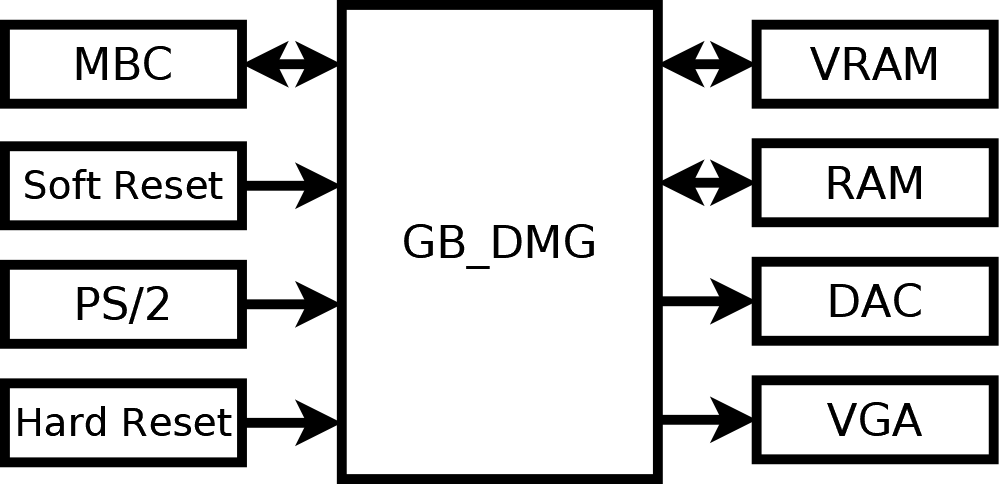
\includegraphics[width=\textwidth, height=0.3\textheight, keepaspectratio=true]{gb_block}
\hypertarget{fig3}{\caption{GameBoy Emulator Layout}}
\end{figure}

\clearpage


\begin{figure}[ht]
\centering
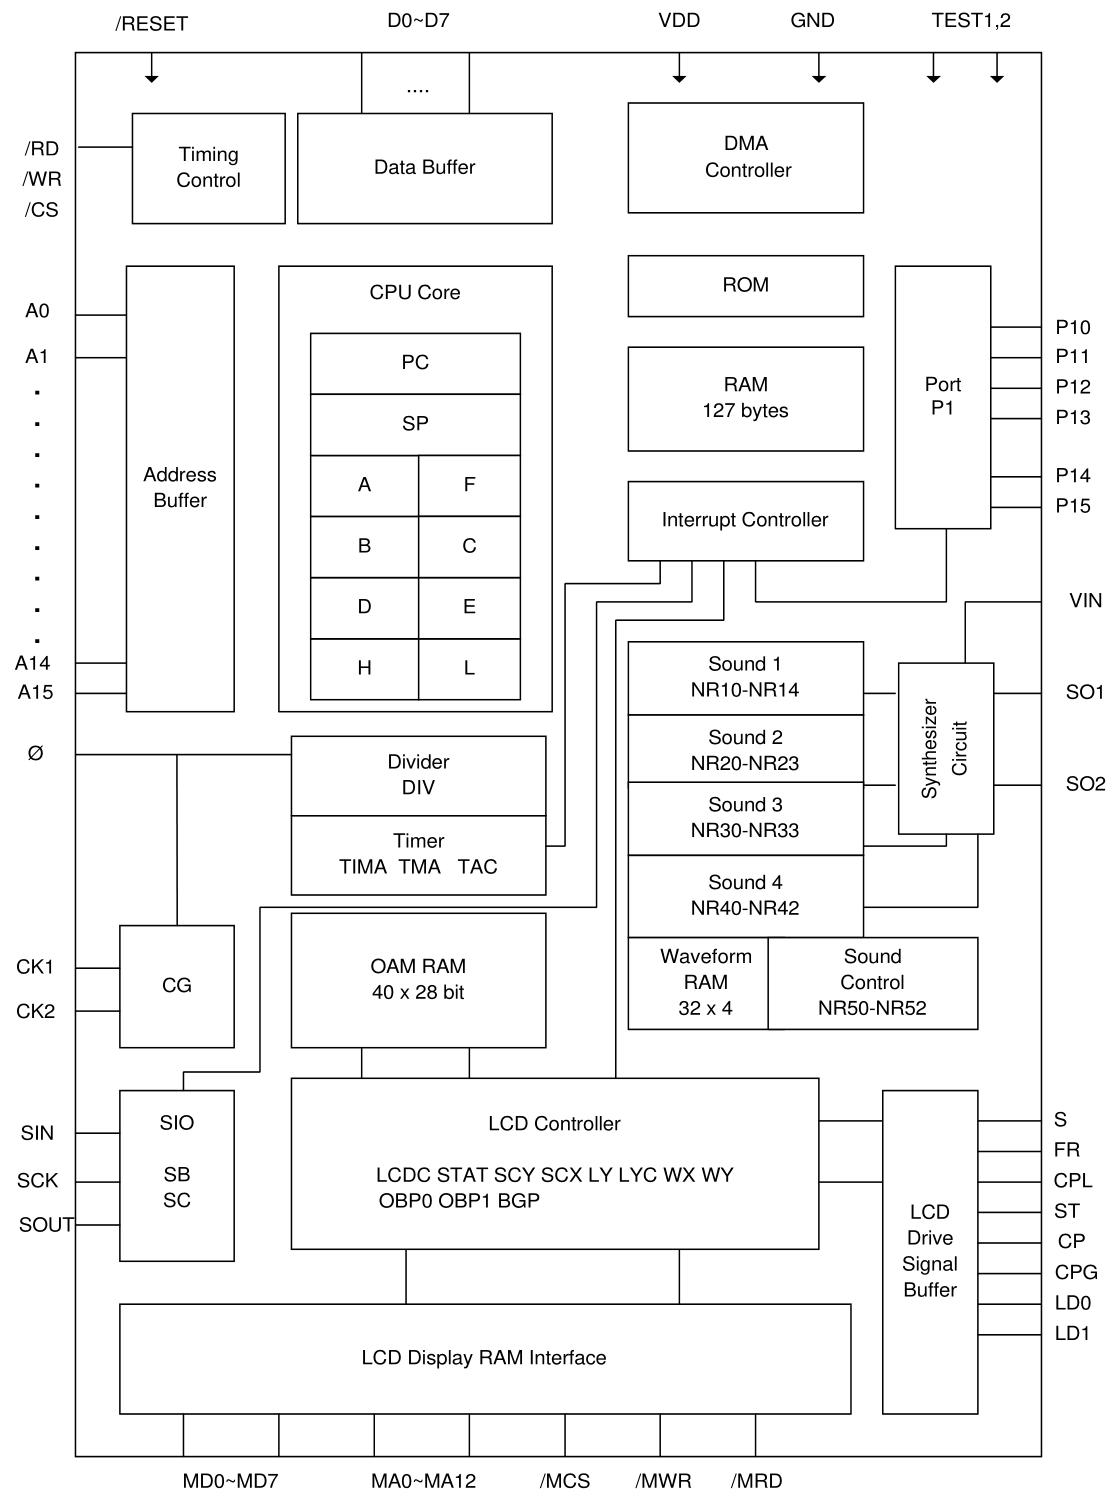
\includegraphics[width=\textwidth, height=0.9\textheight, keepaspectratio=true]{gb_dmg}
\hypertarget{fig4}{\caption{GameBoy DMG Layout}}
\end{figure}

\clearpage

\hypertarget{devplan}{\section{Development Plan}}

The development plan will primarily be divided into two phases: development and testing. The development period has already begun and completion is targeted for the end of May 2nd. The testing period will fill the remaining time. 

\subsection{Development Period}

The development period will focus primarily on translating the specification to SystemVerilog then getting it to a synthesisable and mostly functional state. Each new module under development will have assertions specifying the intended operation embedded and testbenches will be developed using constraint based random verification to validate the modules both independently and together. Each module (beyond basic wrapper and pre-existing modules) will have some extent of testbench infrastructure.

\subsection{Testing Period} 

The testing period will focus on physical testing and verifying that the game in question (Pokemon Red) runs properly on the device. This period will focus on mental model-checking, on-chip testing, and general TLC. It is expected that given the constraints of the project that the game should run respectably on the device at the end of this period.

\subsection{Documentation}

This project will use the documentation provided in Annexes A, B, and C. Additionally the WM8731 Audio DAC datasheet, Phillips I2C specification, and DE1-SOC documentation will be provided. The datasheet for the PS/2 IP Core will also be provided once it is selected.

As for deliverable documentation, an updated Design Description will be provided at the end of the project illustrating the final design.

\clearpage

\hypertarget{annexa}{\section{Annex A: Pan Docs GameBoy Documentation}}

\hypertarget{cpucomp}{\textbf{\underline{CPU Comparision with Z80:}}}
\\ \url{http://gbdev.gg8.se/wiki/articles/CPU_Comparision_with_Z80}

\textbf{\underline{CPU Registers and Flags:}}
\\ \url{http://gbdev.gg8.se/wiki/articles/CPU_Registers_and_Flags}

\textbf{\underline{CPU Instruction Set:}}
\\ \url{http://gbdev.gg8.se/wiki/articles/CPU_Instruction_Set}

\textbf{\hypertarget{memmap}{\underline{Memory Map:}}}
\\ \url{http://gbdev.gg8.se/wiki/articles/Memory_Map}

\textbf{\hypertarget{videosub}{\underline{Video Subsystem:}}}
\\ \url{http://gbdev.gg8.se/wiki/articles/Video_Display}

\textbf{\hypertarget{soundcontrol}{\underline{Audio Subsystem Control:}}}
\\ \url{http://gbdev.gg8.se/wiki/articles/Sound_Controller}

\textbf{\hypertarget{soundhardware}{\underline{Audio Subsystem Hardware:}}}
\\ \url{http://gbdev.gg8.se/wiki/articles/Gameboy_sound_hardware}

\textbf{\hypertarget{interrupt}{\underline{Interrupts:}}}
\\ \url{http://gbdev.gg8.se/wiki/articles/Interrupts}

\textbf{\hypertarget{timer}{\underline{Timer Behaviour:}}}
\\ \url{http://gbdev.gg8.se/wiki/articles/Timer_Obscure_Behaviour}

\textbf{\underline{Power Up Sequence:}}
\\ \url{http://gbdev.gg8.se/wiki/articles/Power_Up_Sequence}

\textbf{\underline{Summary of Subsystem Operations:}}
\\ \url{https://copetti.org/projects/consoles/game-boy/}

\clearpage

\includepdf[pages={30}, frame=true, pagecommand={\hypertarget{annexb}{\section{Annex B: VESA Timing Guidelines}}
\thispagestyle{plain}}, height = 0.9\textheight]{docs/VESA_Timing_Guidelines.pdf}

\clearpage

\hypertarget{annexc}{\part*{Annex C:\\Official GameBoy Documentation}}

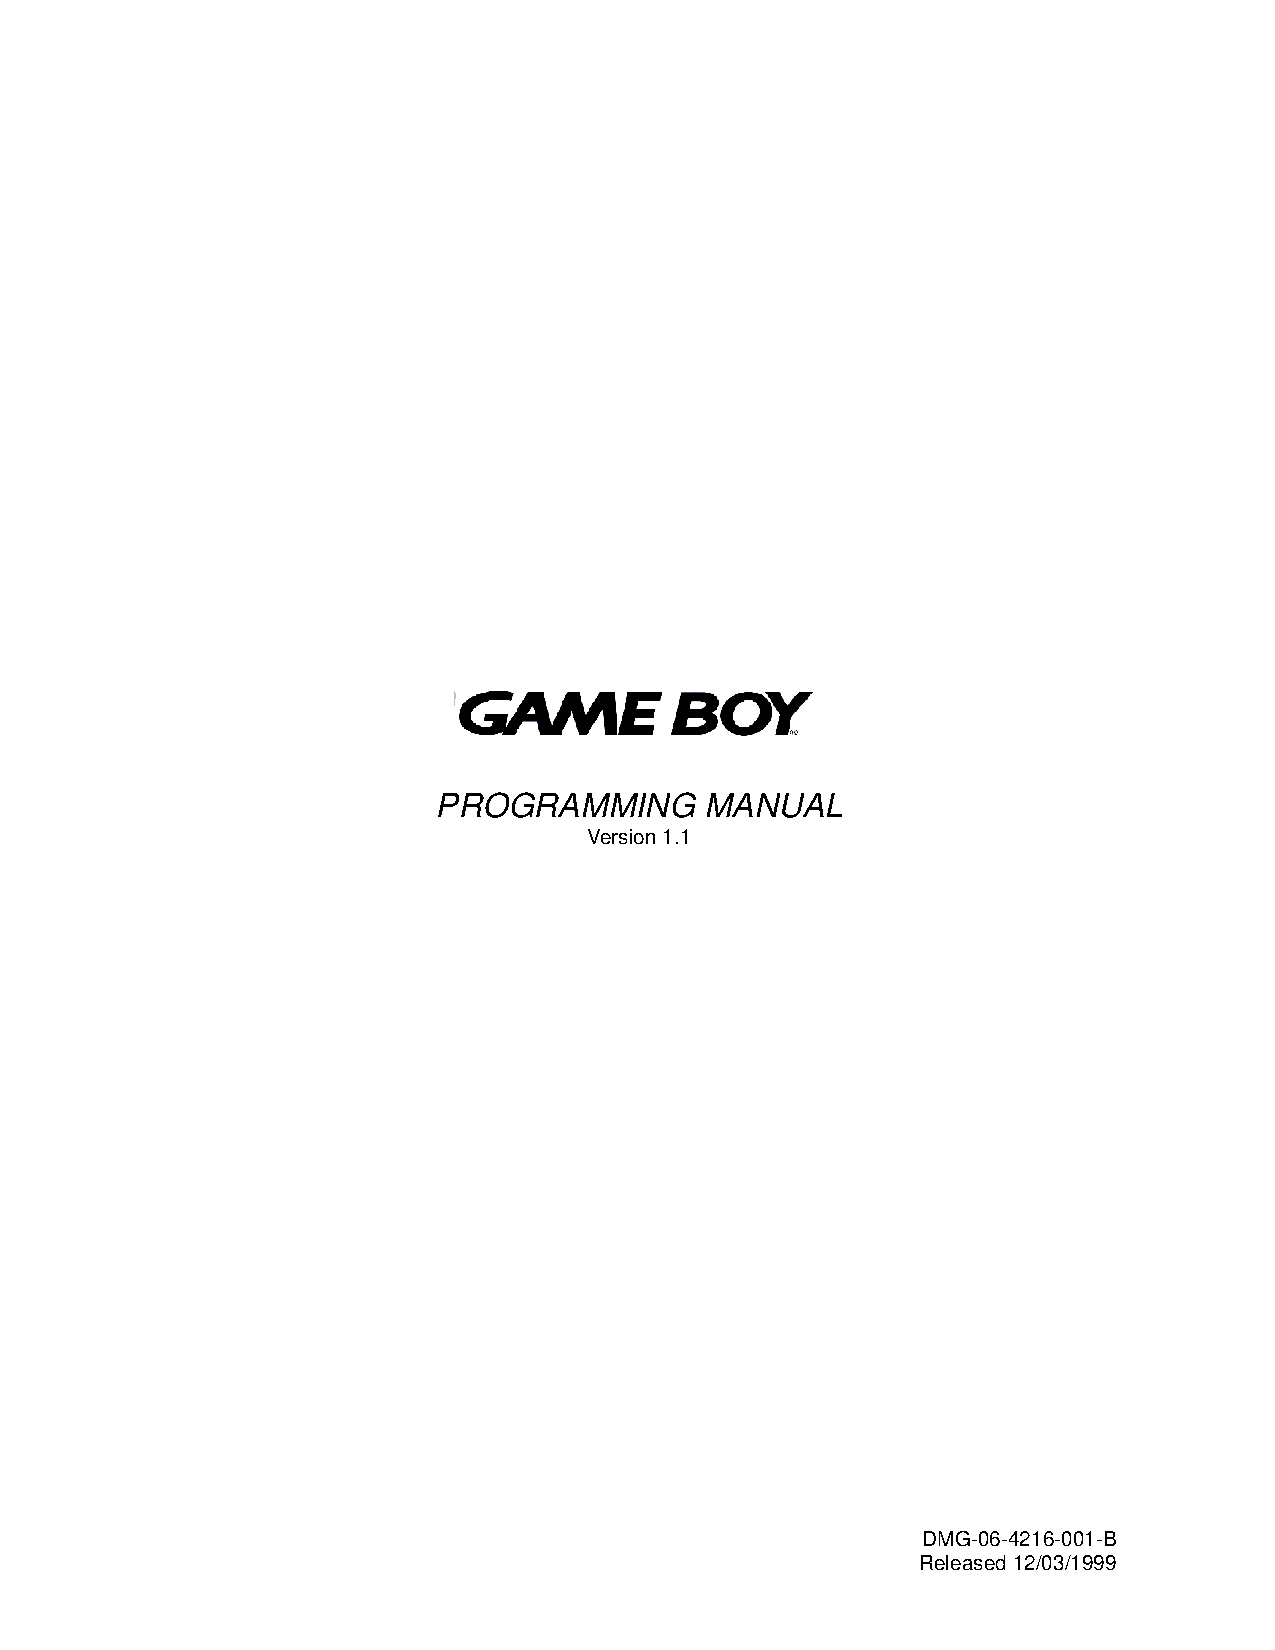
\includepdf[pages={1-136, 215-234,253-283}, frame=true, pagecommand={\thispagestyle{plain}}, height = \textheight]{docs/GameBoy_Manual.pdf}

\end{raggedright}
\end{document}
